\chapter{Solution} \label{chap:solution}

\section*{}

\minitoc \mtcskip \noindent
This chapter describes how the problem presented in Chapter \ref{chap:problem_statement} was solved by stating the solution implemented and the reasons for the choices taken. Section \ref{sec:solution_overview} provides an overview of the developed solution, which is detailed in Section \ref{sec:implementation_details}. Finally, in Section \ref{sec:solution_summary}, a summary of the developed solution is presented, which mentions some limitations of the developed solution and problems that is able to solve.

\section{Overview}\label{sec:solution_overview}

In our solution, we use Node-RED for both (1) defining programs (as flows) and (2) orchestrate the decentralization and send tasks to other devices in the network, acting as a orchestration controller. The devices in the network make themselves known by announcing their address and capabilities to a registry \textit{node} running in Node-RED. Consequently, Node-RED assigns \textit{nodes} to devices taking into account their capabilities and communicates each node's assignment via HTTP. Due to the devices' limitations, they cannot run an instance of Node-RED, so Node-RED needs to translate the \textit{nodes} code in JavaScript to other language that can be interpreted by these devices. 

Node-RED was modified to meet the distributed computation communication demands by replacing the built-in communication by an MQTT-based one. Two main components, as \textit{nodes}, were introduced to the Node-RED palette: (1) the \textit{Registry node} which maintains a list of available devices and their capabilities and, (2) the \textit{Orchestrator node} which partitions and assigns computation tasks to the available devices. Additionally, support was added to Node-RED to generate MicroPython-compatible code from custom \textit{nodes}, \ie code-to-code transformation.

Additionally, a MicroPython-based firmware was developed that is able to receive and run arbitrary Python code scripts generated by Node-RED, and communicate with other devices or Node-RED itself using MQTT. 

An high-level overview of the system can be seen in Fig.~\ref{fig:solution_overview}. Each module will be analyzed in detail in the following sections.

\begin{figure}[h]
    \centering
    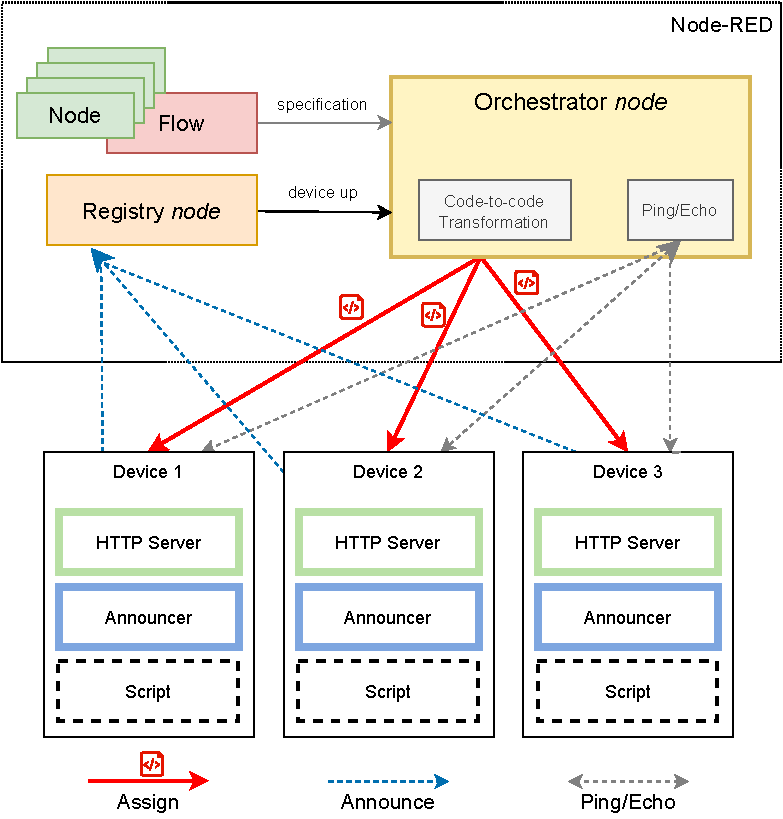
\includegraphics[width=\linewidth]{orchestrator-overview.pdf}
    \caption{Solution's overview, presenting three devices as orchestration \textit{targets}.}
    \label{fig:solution_overview}
\end{figure}

\section{Implementation Details}\label{sec:implementation_details}

The implemented solution consists of two co-dependent modules that are necessary for the functionally of the system. The first module consists of the changes implemented to Node-RED run-time to allow for its decentralization, detailed in Section \ref{sec:node_red_decentralization}. The second module consists of the solution found to take advantage of external devices with limited capabilities, explained in Section \ref{sec:devices_decentralization}.

\subsection{Devices Setup for Decentralization Support}\label{sec:devices_decentralization}

For the purposes of this work we considered constrained devices that are capable of running custom code. Amongst the available hardware solutions, taking into consideration both costs and features, we picked two IoT development devices based on the Espressif Systems ESP32 and ESP8266 systems on chip (SoC)~\cite{esp32,esp8266}. An overview on these devices hardware capabilities is given on Table~\ref{tab:esps}.

\begin{table}[h]
\centering
\begin{tabular}{@{}lll@{}}
\toprule
& \textbf{ESP8266} & \textbf{ESP32}\\ \midrule
MCU & Single-core 32bit & Dual-Core 32bit \\
Frequency & 80 MHz & 160 MHz \\
SRAM & 160kBytes & 512kBytes \\
Flash & SPI, 16MBytes & SPI, 16MBytes \\
802.11 b/g/n WiFi & Yes & Yes \\
Bluetooth & No & Yes \\
Programming Lang.  & \multicolumn{2}{c}{Lua, Python and C} \\ \bottomrule
\end{tabular}
\caption{Comparison between the Espressif Systems ESP32 and ESP8266 systems on chip.}
\label{tab:esps}
\end{table}

The first challenge was to find a way to take advantage of the constrained devices, by making them run arbitrary scripts of code and communicate with other devices. Since both selected devices are able to run MicroPython firmware, Python was the selected programming language. Further, MicroPython already packs a small-footprint HTTP server and packages are available to implement asynchronous operations --- \ie \texttt{uasyncio} --- and MQTT pub-sub communication --- \ie \texttt{MicroPython-mqtt}.

\begin{figure}[h]
    \centering
    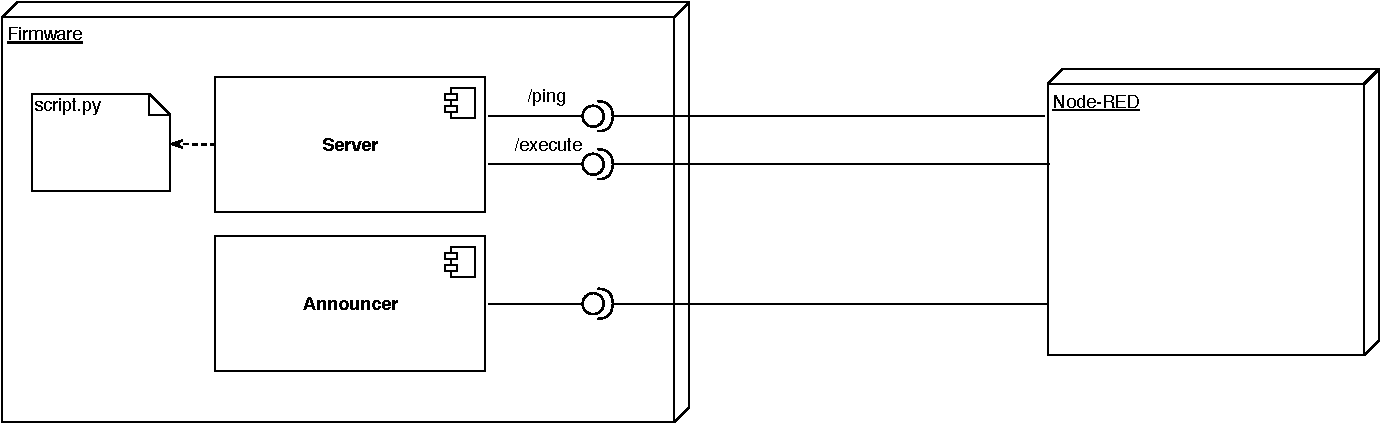
\includegraphics[width=\linewidth]{firmware-component-diagram.pdf}
    \caption{Firmware component diagram.}
    \label{fig:firmware_component_diagram}
\end{figure}

As the devices must be able to receive arbitrary Python scripts (sent by Node-RED) and run them, the HTTP server was used to receive the Python payloads, which are then saved in the device SPI Flash and can be later executed (loaded to the SRAM). Further, the same HTTP server was used to implement an endpoint that returns the state of the device, as well as an announcing mechanism (\cf Section~\ref{sec:registry}). These features built as integral part of the firmware that runs on the devices. An overview of the components of the firmware can be seen in Figure \ref{fig:firmware_component_diagram}.

The firmware also includes a \textsc{fail-safe} mechanism, safeguarding against \textit{Out-of-Memory} errors that may happen during the lifespan of the device (SRAM usage). This mechanism resets all running tasks and recovers the HTTP server and communication channels. This an important feature due to the high probability of these error's occurrence, since the devices have limited memory. 

However, this solution is not without some limitations from which we highlight: (1) the developed firmware only supports MQTT QoS levels 0 and 1 due to \texttt{MicroPython-mqtt} limitations, and (2) ESP8266 severe memory limitations prohibit the use of the \textsc{fail-safe} mechanism if the given script is too big.

\subsection{Decentralized Node-RED Computation}\label{sec:node_red_decentralization}

Node-RED is a centralized tool by design, which takes advantage of events to allow communication between \textit{nodes} in a \textit{flow}. To implement a decentralized architecture, some changes were made to the Node-RED runtime. These changes consisted mainly in (1) implementing a new way of communication between \textit{nodes}, (2) add code-to-code generation features (\ie JavaScript to MicroPython), (3) . These are described in the following paragraphs.

\subsubsection{Node-RED Node-to-Node Communication}\label{sec:mqtt_support}

Node-RED \textit{nodes} communicate using events --- node.js \texttt{EventEmitter}, where a \textit{node} only communicates with \textit{nodes} it is wired to. The communication is one-way only (forward message passing), with the \textit{node} only sending data to the \textit{nodes} it is connected to by output. These output wires are used to access the \textit{nodes} the message must be sent to, and their \texttt{receive()} method is called. This method triggers the event \texttt{emit()} which will the caught by a specific method of each \textit{node}, implementing its own logic.

This implementation is local and JavaScript specific, making it impossible to be used in a decentralized architecture where \textit{nodes} will be executed outside of Node-RED. It was necessary to implement a way of communicating between \textit{nodes} external to Node-RED that could be supported by low capacity devices. The solution found was MQTT, which fits as a good solution by its low-footprint and high-popularity amongst IoT solutions~\cite{soni2017survey}.

Thus, the Node-RED \texttt{Node} class was modified to use MQTT pub-sub communication instead of the in-place communication. Each \textit{node} publish messages to an unique and addressable topic generated at the flow start, to which the next \textit{node} in the \textit{flow} subscribes to. This happens for every \textit{node} with the exception of \textit{producer} \textit{nodes} that only publish messages and \textit{consumers} that only subscribe to topics.

Since the modifications were made at the class (from which every \textit{node} derives from) all the existent \textit{nodes} and sub-\textit{flows} are compatible with this modification without any changes in their code. However, as it will be described next, if we want a node to be orchestrabable, the code of the \textit{nodes} themselves needs to be changed.

\subsubsection{Code Generation}\label{sec:code_generation}

To orchestrate Node-RED \textit{nodes} computation amongst devices there is the need to generate MicroPython-compatible code from the existent JavaScript. Additionally, it is necessary to support multiple \textit{nodes} in one script (\ie condensate), thus a generalized strategy was defined that could fit any type of \textit{node}.

This was accomplished by adding specific code generation methods to each orchestrabable \textit{node}, which provide (1) their functionality, and (2) input/output capabilities. Since every \textit{flow} communication is now MQTT-based, the only input and output a \textit{node} can have is in its topics. A exception to this is in \textit{nodes} that are producers, meaning that they generate input and don't receive it. 

The code generation happens after the \textit{Orchestrator node} defines an assignment between \textit{nodes} and devices. This generation creates a device-specific Python scripts that follows the result of the task assignment procedure (script which can correspond to several \textit{nodes}), adding wrapping code that ties up the script. This wrapping code is responsible for subscribing to all the input topics of all the nodes, stopping the script's processes and forwarding the MQTT messages to the respective node's code.

An example of a Node-RED flow and its respective python script can be seen in Figure \ref{fig:code_generation_flow} and Listing \ref{lst:code_generation}.

\begin{figure}[h]
    \centering
    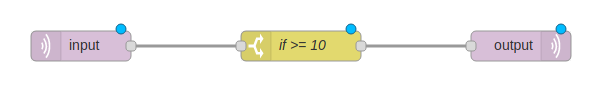
\includegraphics[width=\linewidth]{code-generation-flow.png}
    \caption{Simple Node-RED flow.}
    \label{fig:code_generation_flow}
\end{figure}

\begin{lstlisting}[language=Python, caption={Code generated from the flow presented in Figure \ref{fig:code_generation_flow}.}, captionpos=b, label={lst:code_generation}]
import gc
import sys
import ujson
import uasyncio as asyncio
mqtt_client = None
capabilities = []
client_id = None
nodes_str = "mqttin:3d70bdef542242 mqttout:40d7b1d7aca938 if:fd3cf13026958"
nodes_id = ["3d70bdef542242","40d7b1d7aca938","fd3cf13026958"]
input_topics = ["input","topic1_node","topic0_node"]
output_topics = ["topic0_node","topic1_node"]

import ubinascii
input_topics_3d70bdef542242 = ["input"]
output_topics_3d70bdef542242 = ["topic0_node"]
node_datatype_3d70bdef542242 = "auto"
node_qos_3d70bdef542242 = 2

def on_input_3d70bdef542242(topic, msg, retained):
    try:
        if node_datatype_3d70bdef542242 == "base64":
            msg = str(ubinascii.b2a_base64(msg))
        elif node_datatype_3d70bdef542242 == "utf8":
            msg = msg.encode("utf-8")
        elif node_datatype_3d70bdef542242 == "json":
            msg = ujson.loads(str(msg))
    finally:
        msg = dict(
            topic=topic,
            payload=msg,
            device_id=client_id
            qos=node_qos_3d70bdef542242,
            retain=retained
        )
        loop = asyncio.get_event_loop()
        loop.create_task(
            on_output(
                ujson.dumps(msg),
                output_topics_3d70bdef542242
            )
        )

import ujson
input_topics_40d7b1d7aca938 = ["topic1_node"]
output_topics_40d7b1d7aca938 = ["output"]

def on_input_40d7b1d7aca938(topic, msg, retained):
    try:
        msg = ujson.loads(msg)
    else:
        msg = dict(
            topic=topic,
            payload=msg["payload"],
            device_id=client_id
        )            
    loop = asyncio.get_event_loop()
    loop.create_task(
        on_output(
            ujson.dumps(msg),
            output_topics_40d7b1d7aca938
        )
    )

input_topics_fd3cf13026958 = ["topic0_node"]
output_topics_fd3cf13026958 = ["topic1_node"]
property_fd3cf13026958 = "payload"

def if_rule_fd3cf13026958_0(a, b = 10):
    a = int(a)
    return a >= b
def if_function_fd3cf13026958(a):
    res = if_rule_fd3cf13026958_0(a)
    return '%s' % res

def get_property_value_fd3cf13026958(msg):
    properties = property_fd3cf13026958.split(".")
    payload = ujson.loads(msg)

    for property in properties:
        try:
            payload = ujson.loads(payload)
            if payload[property]:
                payload = payload[property]
            else:
                break
        except:
            break
    return payload

def on_input_fd3cf13026958(topic, msg, retained):
    msg = get_property_value_fd3cf13026958(msg)
    res = if_function_fd3cf13026958(msg)
    res = dict(
        payload=res,
        device_id=client_id
    )
    loop = asyncio.get_event_loop()
    loop.create_task(
        on_output(
            ujson.dumps(res),
            output_topics_fd3cf13026958
        )
    )
    return

def on_input(topic, msg, retained):
    topic = topic.decode()
    if topic in input_topics_3d70bdef542242:
        on_input_3d70bdef542242(topic, msg, retained)
    elif topic in input_topics_40d7b1d7aca938:
        on_input_40d7b1d7aca938(topic, msg, retained)
    elif topic in input_topics_fd3cf13026958:
        on_input_fd3cf13026958(topic, msg, retained)

async def conn_han(client):
    for input_topic in input_topics:
        await client.subscribe(input_topic, 1)

async def on_output(msg, output):
    for output_topic in output:
        await mqtt_client.publish(output_topic, msg, qos = 1)

def get_nodes():
    return nodes_str

def stop():
    for id in nodes_id:
        func_name = "stop_" + id
        if func_name in globals():
            getattr(sys.modules[__name__], func_name)()

async def exec(mqtt_c, capabilities_array, c_id):
    global mqtt_client
    global capabilities
    global client_id
    mqtt_client = mqtt_c
    capabilities = capabilities_array
    client_id = c_id
    for id in nodes_id:
        func_name = "exec_" + id
        if func_name in globals():
            getattr(sys.modules[__name__], func_name)()
    return
\end{lstlisting}

However, there are limitations to this solution. If two consecutive \textit{nodes} are assigned to the same device, the communication between them is still dependent on MQTT. This is not an ideal solution, since one \textit{node} could call the other through code, passing its output as arguments.

\subsubsection{Custom Nodes}\label{sec:custom_nodes}

As previously mentioned, all the existent \textit{nodes} are compatible with the modified Node-RED. Nonetheless, for a \textit{node} to be orchestrabable, it must be modified to comply with the code generation needs. As proof-of-concept, the following \textit{nodes} were modified or created to be orchestrabable:
\begin{description}
    \item[\texttt{IF} \textit{node}] which receives an input and verifies if it complies with all the given rules, returning true or false;
    \item[\texttt{AND} \textit{node}] which receives a given number of inputs and verifies if all of them are true or false, returning the corresponding boolean;
    \item[\texttt{TEMP-HUM} \textit{node}] that read the temperature and humidity from a DHT sensor present in a specific pin;
    \item[\texttt{FAIL} \textit{node}] that raises a MemoryError exception;
    \item[\texttt{NOP} \textit{node}] that simply redirects the received message in its input to its output;
    \item[\texttt{MQTT IN} and \texttt{MQTT OUT} \textit{nodes}] that subscribe and publish MQTT topics, respectively.
\end{description}

Additionally, each of these \textit{nodes} has two accessible properties: Predicates and Priorities. Similar to the Kubernetes logic of assigning containers to machines~\cite{burns2018managing}, the predicates dictate constraints that cannot be violated, and priorities are requests that are advisable and recommended but can be violated if impossible to comply. 

These \textit{nodes} provide enough functionality to wire simple \textit{smart home} scenarios and validate our approach.

\subsubsection{Device Registry}
\label{sec:registry}

IoT systems are typically built on top of heterogeneous parts, with different capabilities and resources and their network can be highly-dynamic (devices appearing and disappearing according to factors such as battery levels, hardware/software failures and communication interference). In order to maintain a \textit{list} of the available devices in the network along with their capabilities there is a need for a Device Registry~\cite{Ramadas17}.

When a device becomes available it sends information about itself to a MQTT topic. This information contains the device's IP address, their capabilities and their status --- if the device has failed before. In its turn, Node-RED contains a \textit{Registry node} that listens to the announcements MQTT topics and saves the devices information. If this \textit{node} is connected to an \textit{Orchestrator node}, each new device is communicated so that the orchestration can be updated.

When a device has an \textsc{Out-of-Memory} error, it triggers a \textsc{fail-safe}, where it reboots the HTTP server, stops running any script and restarts all communications. After this action, the device announces itself again but with a flag that indicates that it has failed. This way, the \textit{Orchestrator node} knows that a device is active but not running any code, and that it is possible that it failed due to too much work. In that case, it can dynamically adapt and assign less \textit{nodes} to the device, reducing the chances of causing another \textsc{Out-of-Memory} error.

\subsubsection{Computation Decentralization}\label{sec:node_red_computation_decentralization}

Node-RED must be capable of distribute computation amongst available resources (\ie devices), thus, given a set of tasks, it must assign them to available devices, ensuring that they will be performed.

The requirements to achieve this are two-fold: first, a \textit{node} should act as coordinator, which when provided with an available devices list, along with their respective capabilities (\cf Section~\ref{sec:registry}), should decide which device should execute specific computation \textit{nodes} --- \textit{Orchestrator node} --- and, second, the orchestrabable \textit{nodes} should provide both Predicates and Priorities that must be meet to assure their correct execution (\cf Section~\ref{sec:custom_nodes}).

\begin{algorithm}
\Input{deviceList}
\Output{bestDevice}
\BlankLine
\Init{node: $node$\\
     bestIndex: $0$\\
     bestDevice: $null$
    }
\BlankLine
\OnInput{
    \For{$device$ \textbf{in} $deviceList$}{
        \If{\textbf{not} \textbf{all} $node$.$predicates$ \textbf{in} $device$.$tags$}{
            \Return
        }
        
        $intersectionIndex$ $\gets$ $\sum{node.priorities \in \text{device.tags}}$ / $\sum{priorities\in\text{node}}$
        
        $nodesPerDevice$ $\gets$ $\sum{nodes \in \text{device}}$
        
        $nodesPrioritiesPerDeviceRatio$ $\gets$ $\sum{node.priorities \in \text{device.tags}}$ / $\sum{device \in \text{tags}}$ 
        
        $matchIndex$ $\gets$ $intersectionIndex * 0.5 + (1/nodesPerDevice + 1) * 0.4 + nodesPrioritiesPerDeviceRatio * 0.1$
        
        \If{$matchIndex$ > $bestIndex$}{
            $bestIndex$ $\gets$ $matchIndex$  \Comment*[r]{Device is best for node}
            $bestDevice$ $\gets$ $device$
        }
    }
    \Return $bestDevice$
}
\caption{Greedy algorithm for \textit{node} assignment.}
\label{code:greedyassignment}
\end{algorithm}

The assigning algorithm uses the devices capabilities and each node's Predicates and Priorities to assign \textit{nodes} to devices. With a greedy approach, the algorithm filters the devices that comply with each node's predicates and assigns the one with a higher value of a heuristic, \cf Algorithm~\ref{code:greedyassignment}. This heuristic takes into account the number of priorities the device can provide, as well as the number of already assigned \textit{nodes} the device has. The goal is to assign each \textit{node} to the best possible device, spreading the tasks through all the available devices. An example of a possible assignment can be seen in Figure \ref{fig:assigment_example}, where the assignment matches the nodes' priorities with the devices' tags while spreading the nodes over the available devices.

\begin{figure}[h]
\centering
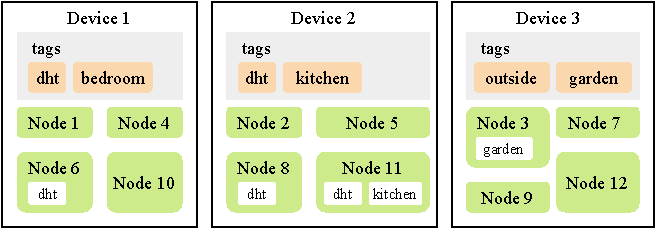
\includegraphics[width=\linewidth]{assignment_example.pdf}
\caption[Node assignment example.]{Node assignment example.}\label{fig:assigment_example}
\end{figure}

After assigning all \textit{nodes} to a specific device, a code script is generated for each device (\cf Section~\ref{sec:code_generation}). Due to the constrained memory of the devices, the quantity of \textit{nodes} assigned to a device may exceed their resources. In that case, the device will \textsc{fail-safe} and return an error to the assignment request. The orchestrator will receive this information and repeat the process, assigning less \textit{nodes} to the devices that returned an \textsc{Out-of-Memory} error. If a device does not return any response, the orchestrator will assume that the device is unavailable and not assign any \textit{node} to it.

The \textit{Orchestrator node} can be triggered --- proceeding to a system (re)orchestration --- by the following events: (1) start of the system, when there is already a defined flow in the configuration, the assignment start after a period of 3 seconds, to give time for the devices to be registered by the registry node; (2) deployment of the entire flow using the Node-RED editor or API; (3) appearance of a new device detected by the \textit{Registry node}; (4) failure or recovery of a device, which, working as a complement to the \textit{Registry node}, is detected using \textsc{Ping/Echo} pattern~\cite{Scott2009} which periodically \textit{pings} the devices in the system to assert their operational status. A visual representation of this events can be seen in Figure \ref{fig:sequence_diagram}. 

\begin{figure}[h]
\centering
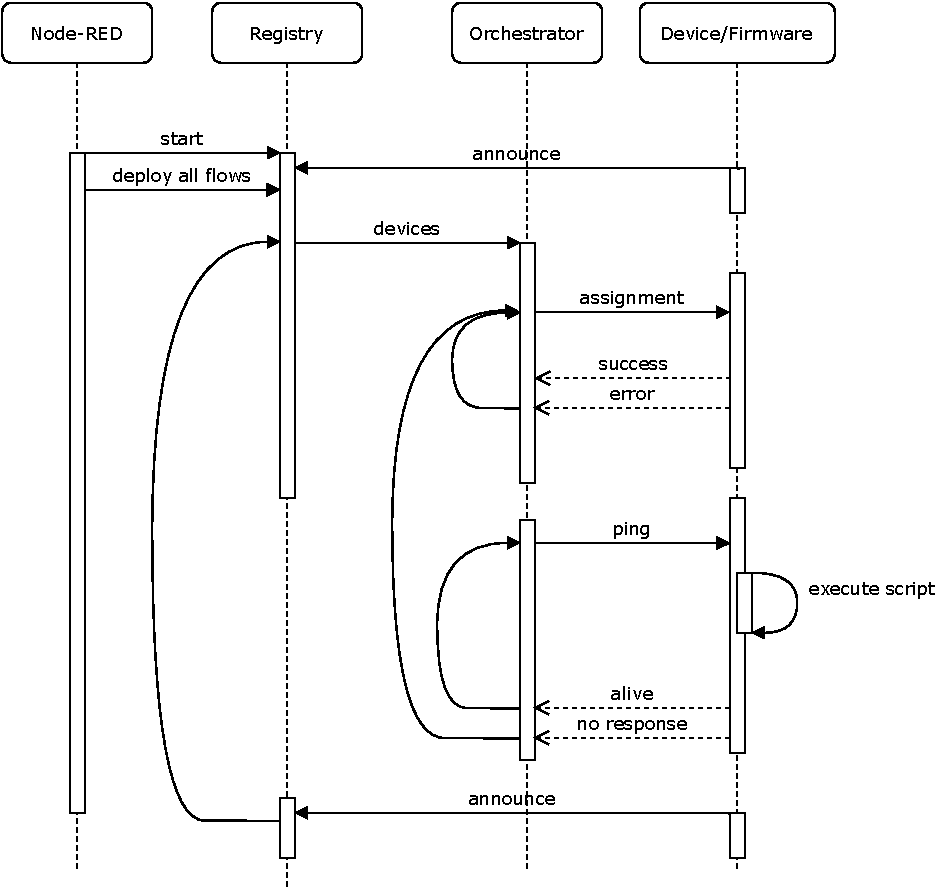
\includegraphics[width=\linewidth, height=12cm, keepaspectratio]{sequence-diagram.pdf}
\caption[Sequence of events for orchestration.]{Sequence of events for orchestration.}\label{fig:sequence_diagram}
\end{figure}

There are, however, some limitations in the assignment process, mostly due to the algorithm used. There are cases when the resulting assignment is not the best possible solution, and sometimes the orchestration can fail completely since it can not comply with the constraints imposed by nodes. As an example, given a scenario where the number of devices is small for the quantity of nodes, it is possible that the devices are kept at the limit of their resources, \ie memory. If there is a \textit{node} which constraints can only be complied by one device, but that one device already has the maximum number of \textit{nodes} it can handle, the assignment is not possible.

In addition to this, the assignment algorithm does not take into account the connections between \textit{nodes}. As mentioned before, sequential nodes in the same device communicate via MQTT topics instead of calling themselves through code. However, if that was not the case, it would be advantageous if sequential \textit{nodes} were assigned to the same device. This would allow better performance, less communication load and less dependency on an external MQTT client.

\subsection{Summary}\label{sec:solution_summary}

The developed solution covers all the desired requirements established in Section \ref{sec:desiderata}. It identifies available devices in the network and decentralizes the given computation through them. It translates each computation task into something comprehensible for the devices. In addition to this, the developed system maintains the state, adapting to any change in the availability and constraints of the devices.

However, there are some limitations that are not trivial. Some of them were already identified in previous sections: (a) the number of \textit{nodes} that support MicroPython code generation is small, (b) there is a chance of duplicate MQTT messages that is not being handled, (c) the (re)orchestration using the editor or API is only possible by deploying the entire instance, and not specific flows or nodes, (d) \textit{node} assignment does not favor the assigment of sequential nodes, which would improve efficienty if (e) the script generation did not force all communications between nodes to be through MQTT, instead of allowing a node to call other through code, passing its output as parameters.

Despite the limitations, the developed solution solves the issues identified in Section \ref{sec:current_issues} and provides a decentralized option to a previously centralized product.